\chapter{Implementation}

\section{Application Architecture}

\newpage
\section{Relational Schema}

In order to design the relational schema for the database, we first have to pose the question: what information is relevant to a repository?
Immediately things like the repository name or number of commits come to mind.
Although the introduction only briefly skimmed over some examples of useful data, there are other kinds of metrics based on which researchers may want to limit their selection.
The following is a list of all the data that we have chosen to mine for repositories, as well as an explanation on why they are key characteristics of a project:
\begin{itemize}
    \item \textit{The full repository name, formatted as:} \code{user/repo_name}
    \\Multiple repositories from different owners can have the same name (which makes sense to accommodate forks), but a single user can't create multiple repositories of the same name.
    \item \textit{An indication as to whether a project is a fork of an existing project.}
    \\Forking is central to the Git ecosystem. However in some cases, researchers may want to exclude forks when sampling, as they contain little to no modifications made on the original. Due to how easily they can be created, ``forks with no changes'' may not harbor any useful information to a study, and only serve to bloat a dataset~\cite{FORKS}. On the other hand, researchers may also want to limit the study to only forks of a popular project, with the goal of observing which features of the original may have changed across various forks.
    \item \textit{The number of commits.}
    \\The number of commits is by far the most commonly observed attribute for determining the scope of a project, as they equate to checkpoints in development. It is very common for ``toy projects'' or repositories misusing GitHub as an online storage service to have a low number of commits, which is why they should be filtered out during selection.
    \item \textit{The number of branches.}
    \\Branches represent several lines in development of a software project~\cite{GIT}. They too are good indicators of project scope, as most serious projects use more than the single default branch.
    \item \textit{The number of releases.}
    \\Releases are GitHub's method of packaging and providing software to users~\cite{GITHUBHELP}. Due to the feature being mostly utilised in bigger projects, the number of releases can also be used as a filter for determining how ``big'' a project is.
    \item \textit{The number of contributors.}
    \\As the name suggests, project contributors are GitHub users who have contributed to a project, albeit not as part of the core development team~\cite{GITHUBHELP}. A high contributor count in a public repository is a good indication of how much the community is engaged in a project. It should be of no surprise that personal projects tend not to have high contributor counts.
    \item \textit{The number of watchers.}
    \\The watchers of a public repository are users who have asked to be notified of activity in a repository, but have not become collaborators~\cite{METRICSWATCHERS}. Watchers can be interpreted as an extension to contributors. Although not contributing to projects in a direct way, they tend to be engaged in the discussions surrounding its development, some even going so far as to becoming future contributors~\cite{WATCHERS14}.
    \item \textit{The number of stars.}
    \\Stars were introduced in 2012 as an alternative way of keeping track of interesting projects without receiving notifications~\cite{STARS}. In essence, a project's star count is attributed to its notoriety on the platform. Given how the default sorting order for both the Advanced Search and API is by stars, projects with higher star counts appear first in searches, making them more popular.
\end{itemize}

%TODO Comments on auxiliary data like branch name, commit SHA, homepage, license...

\begin{figure}[ht!]
    \centering
    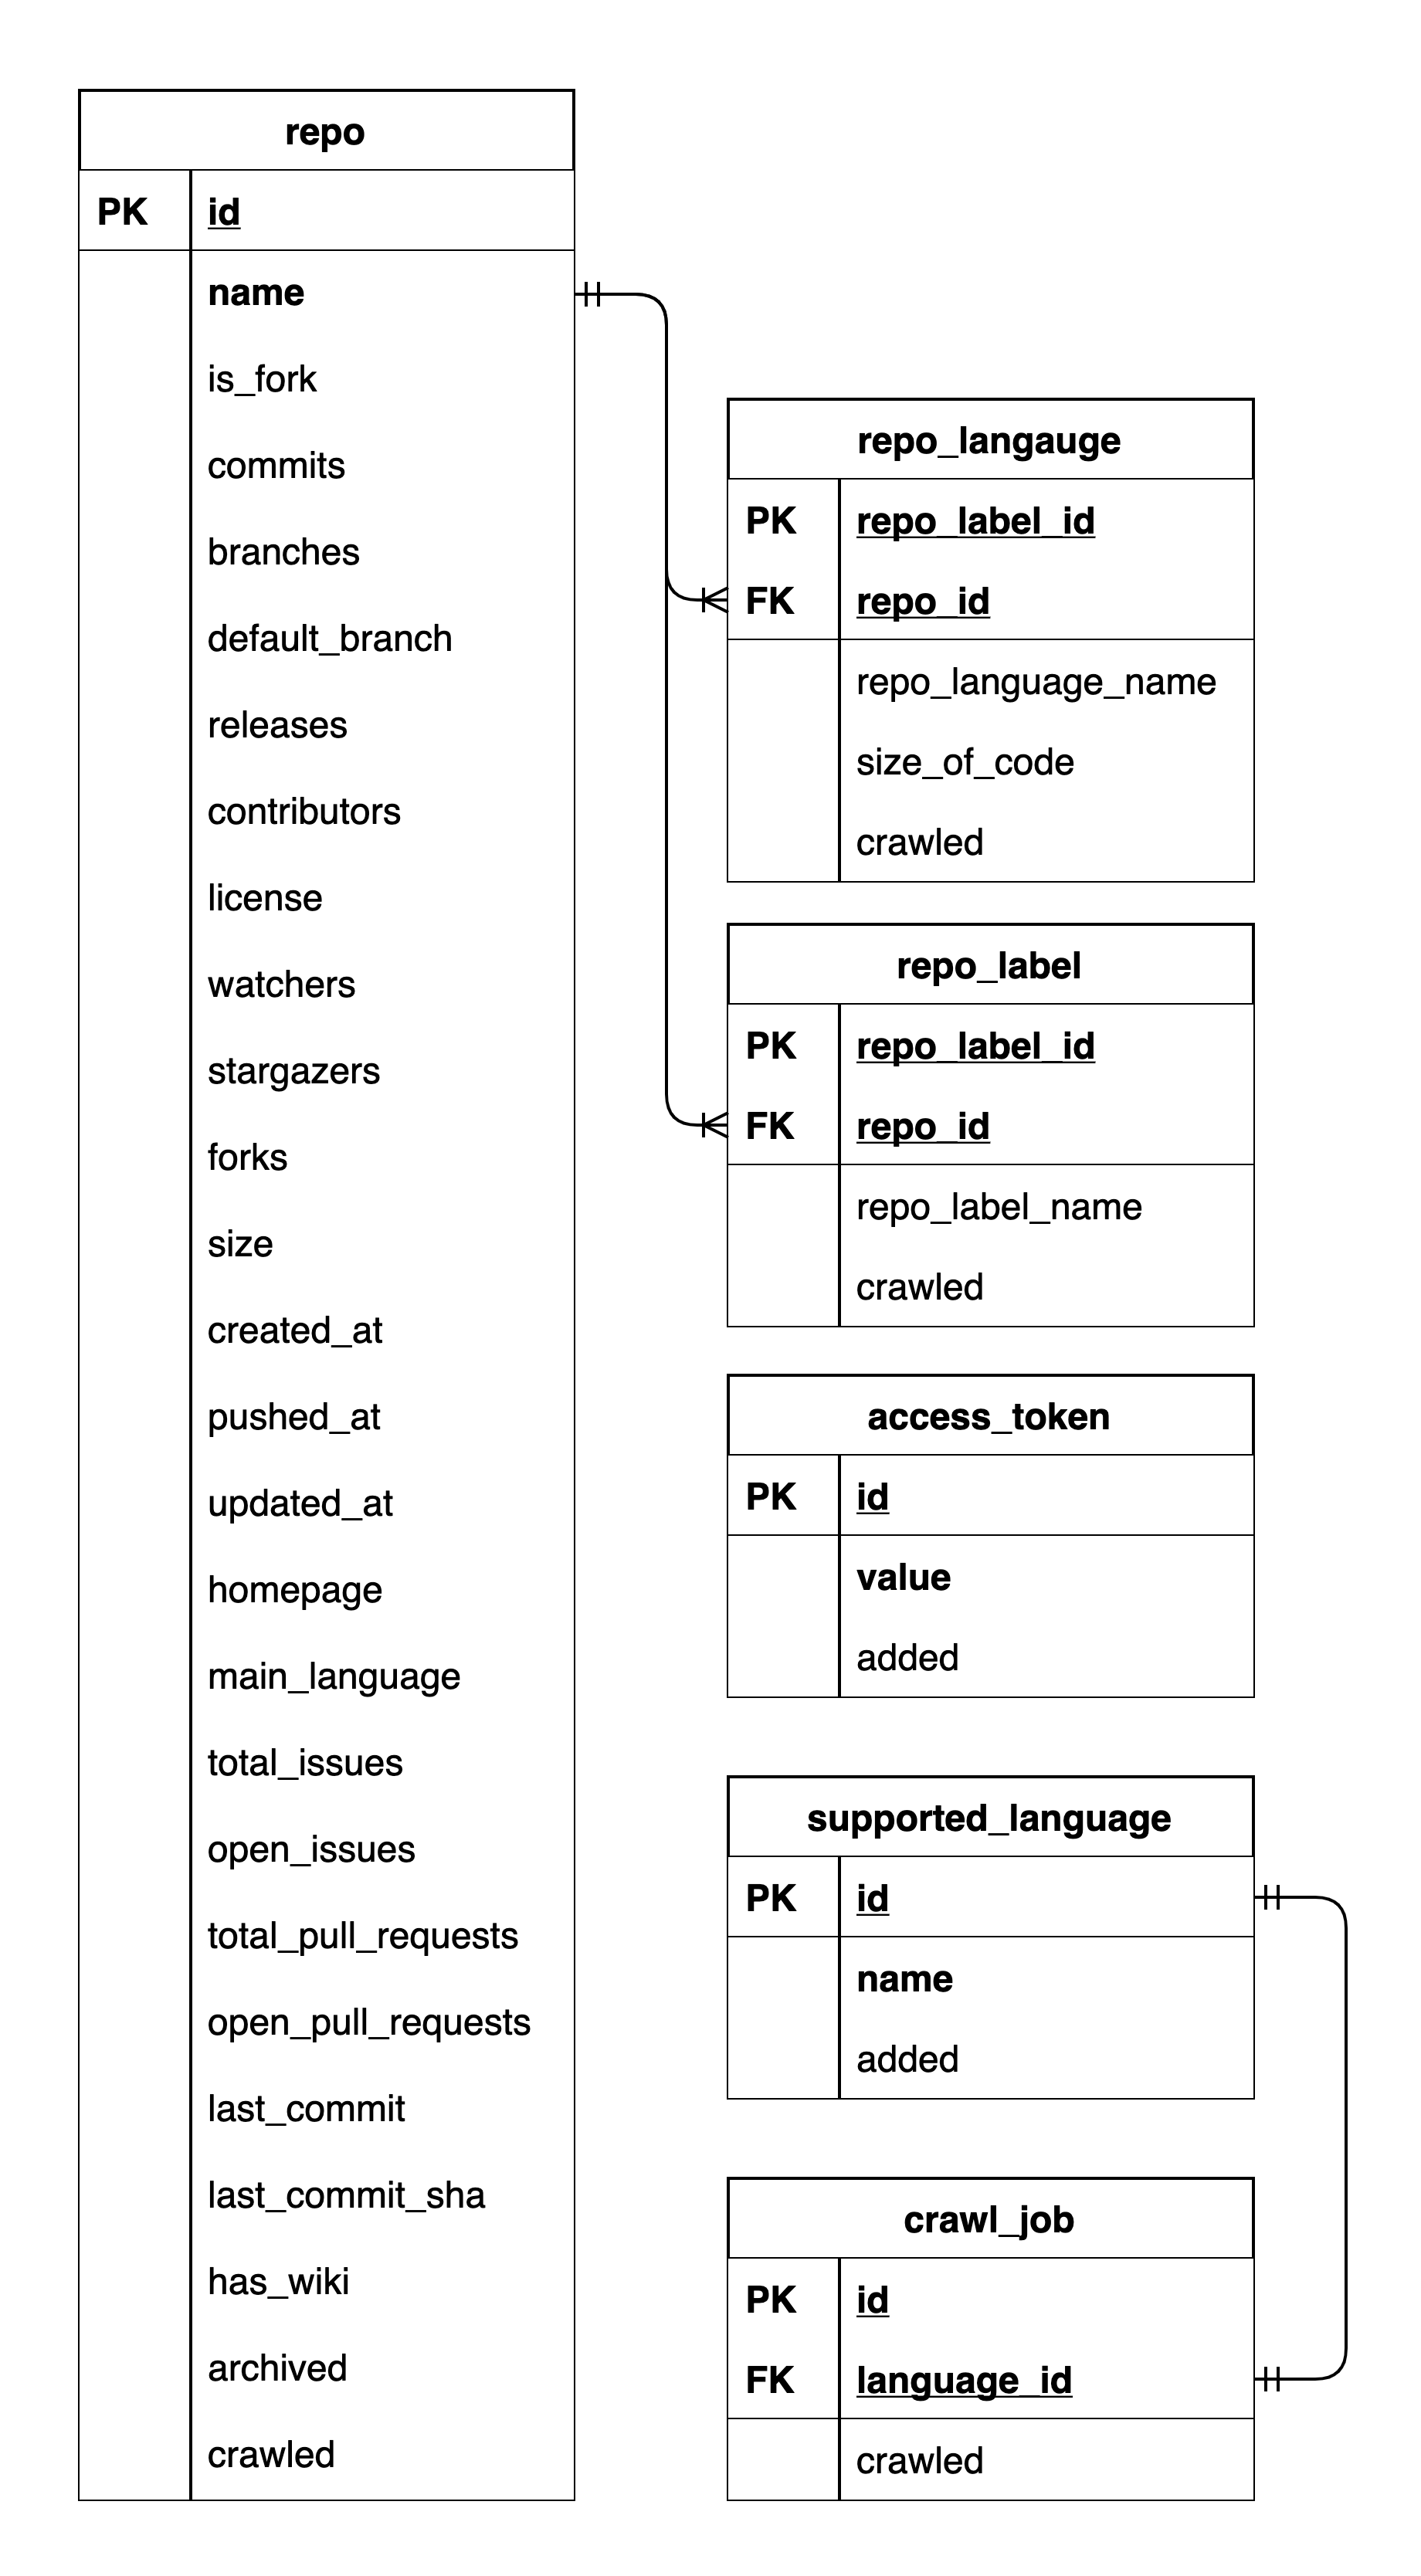
\includegraphics[width=0.7\linewidth]{relational}
    \caption{The relational schema of the database}
\end{figure}

\newpage
\section{The Mining Algorithm}

The mining algorithm is the core of our search engine.
In broad terms, the miner is responsible for mining all the public projects written in a certain language, from a set of languages supported by the app.
Once all the repositories have been mined for one specific language, the miner moves on to the next one.
It's important to note that the miner currently prioritises repositories consisting predominantly of code written in more popular languages such as JavaScript, Python and C++.

The mining algorithm works as follows:
\begin{itemize}
    \item It first looks at the \textit{CrawlJob} table of the database. Since that table indicates the date up to which repositories were mined for a particular language, it uses that information to limit the crawl interval. If no prior ``crawl jobs'' exist, then \textit{January 1st 2008} is chosen as the starting date for the mine, selecting one of the supported languages to crawl first. However if there were prior ``crawl jobs'' for particular languages, then the crawler would simply resume crawling from the date it has acquired information to so far. Although the crawling interval lower bound would either be the start of 2008 or the date that data was mined up to so far, the upper bound would always be the time at which the crawl job was started.
    \item The application then makes a call to the GitHub API, requesting all public projects (fork projects included) created within the aforementioned time interval of a language. By analysing GitHub's response:
    \begin{itemize}
        \item If the number of repositories returned matching this criteria is greater than 1000, then the time interval is split in half, and the API call is repeated for each of the new intervals;
        \item If the number of repositories returned matching this criteria is less than or equal to 1000, then we iterate over each of the results, making additional API calls to retrieve the labels and languages of each of the repositories, as well as scraping the repository web pages for any of the data not obtainable by the API\@. Once all the auxiliary data has been acquired, the date value for the crawl job table for that language is updated to the interval upper bound.
    \end{itemize}
\end{itemize}